\documentclass{article}

\usepackage{tikz}
\usetikzlibrary{external}
\usetikzlibrary{decorations.pathmorphing}
\usetikzlibrary{decorations.markings}
\usetikzlibrary{shapes.arrows}
\usetikzlibrary{arrows}

\usetikzlibrary{positioning,fit,calc}
\usetikzlibrary{arrows.meta}
\usetikzlibrary{calc,fadings,decorations.pathreplacing}
%\usetikzlibrary{arrows.spaced}
\usetikzlibrary{decorations.pathmorphing}

\usepackage[compat=1.1.0]{tikz-feynman}

\usepackage{varwidth}
\usepackage{epstopdf}
\usepackage{amssymb}
\usepackage{relsize}

\tikzset{external/force remake}
\tikzexternalize % activate!

\begin{document}


\begin{center}
   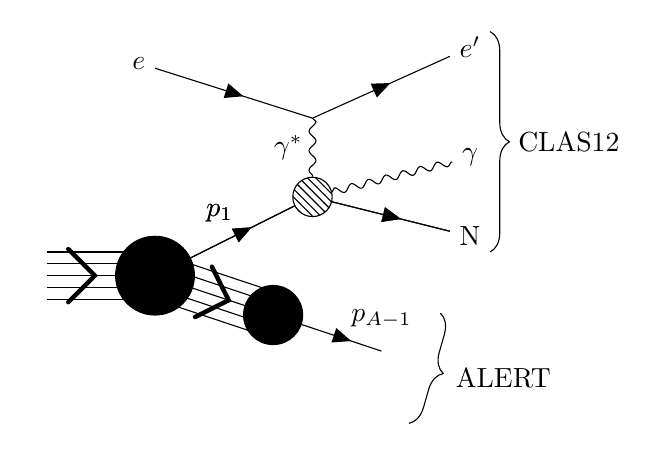
\begin{tikzpicture}
      \begin{feynman}
         \vertex                                            (n0) {};
         \vertex[large, blob, fill=black,right=1.5cm of n0] (n1) {};

         % incoming A nucleons
         \vertex[above = 0.15cm of n0]  (n01){~};
         \vertex[above = 0.30cm of n0]  (n02){~};
         \vertex[above = 0.45cm of n0]  (n03){~};
         \vertex[below = 0.15cm of n0]  (n04){~};
         \vertex[below = 0.30cm of n0]  (n05){~};
         \vertex[below = 0.45cm of n0]  (n06){~};

         \vertex[above = 0.15cm of n1]  (n11){~};
         \vertex[above = 0.30cm of n1]  (n12){~};
         \vertex[above = 0.45cm of n1]  (n13){~};
         \vertex[below = 0.15cm of n1]  (n14){~};
         \vertex[below = 0.30cm of n1]  (n15){~};
         \vertex[below = 0.45cm of n1]  (n16){~};

         \vertex[blob, fill=black, below right=0.5cm and 1.5cm of n1]            
         (n2) {};
         %\vertex[label={[label distance=0.2cm]-130:label},blob, fill=black, 

         \vertex[below right=0.5cm and 1.5cm of n11]  (n21) {};
         \vertex[below right=0.5cm and 1.5cm of n12]  (n22) {};
         \vertex[below right=0.5cm and 1.5cm of n13]  (n23) {};
         \vertex[below right=0.5cm and 1.5cm of n14]  (n24) {};
         \vertex[below right=0.5cm and 1.5cm of n15]  (n25) {};
         \vertex[below right=0.5cm and 1.5cm of n16]  (n26) {};

         \vertex[below right=0.5cm and 1.5cm of n2]      (n3) {};

         %dvcs vertex
         \vertex[small, blob, above right=1.0cm and 2.0cm of n1] (a0) {};

         % e,e'gamma vertex 
         \vertex[above=1.0cm of a0]                  (q0);

         \vertex[below right=0.5cm and 2.0cm of a0]  (a1) {N};
         \vertex[above=1.0cm of a1]                  (q1){\(\gamma\)};

         % electron
         \vertex[above left=0.5cm and 2.0cm of q0]  (e0) {\(e\)};
         \vertex[above=1.4 of q1]   (e1) {\(e^{\prime}\)};

         \diagram*{
            (e0) -- [fermion] (q0) -- [fermion] (e1),
            (n1) -- [fermion, edge label=\(p_1\)] (a0) -- [fermion] (a1),
            (n1) -- [fermion, edge label=\(p_1\)] (a0) -- [fermion] (a1),
            (a0) -- [photon, edge label = \(\gamma^{*}\)] (q0),
            (q1) -- [photon] (a0),
            (n01) --  (n11)  --  (n21),
            (n02) --  (n12)  --  (n22),
            %(n03) --  (n13) --  (n23),
            (n04) --  (n14)  --  (n24),
            (n05) --  (n15)  --  (n25),
            %(n06) --  (n16) ,
            (n0) -- [plain,arrow size=6pt, postaction={decorate}, 
            decoration={markings, mark=at position 0.75 with 
         {\arrow[scale=4]{angle 90}}}] (n1) --
         [plain,arrow size=6pt, postaction={decorate}, decoration={markings, 
         mark=at position 0.75 with {\arrow[scale=4]{angle 90}}}] (n2) -- 
         [fermion, edge label = \(p_{A-1}\)] (n3),
         };

         % alert detection
         \draw [decoration={brace,amplitude=7pt}, decorate]
         ($(n3.north east)+(0.5cm,0.4cm)$) -- ++(-0.4cm,-1.4cm);
         \node[] at ($(n3.east)+(1.3cm,-0.3cm)$) {ALERT};

         % CLAS12 detection
         \draw [decoration={brace,amplitude=7pt}, decorate]
         ($(e1.east)+(0.0cm,0.2cm)$) -- ++(-0.0cm,-2.8cm);
         \node[] at ($(e1.east)+(1.0cm,-1.2cm)$) {CLAS12};

      \end{feynman}
   \end{tikzpicture}
\end{center}

\begin{center}
   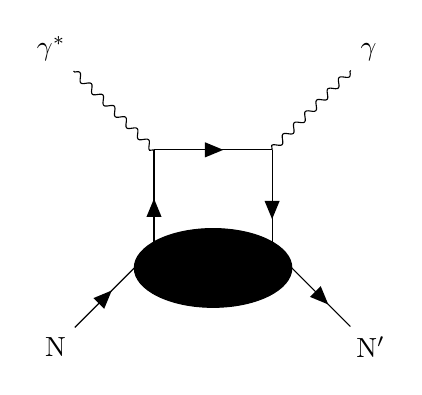
\begin{tikzpicture}
      \begin{feynman}
         \vertex (p1) at (0,0) {N};
         \vertex[above right=1cm and 2.0cm of p1] (a2) { };
         \vertex[below right=1cm and 2.0cm of a2] (p2) {N\(^{\prime}\)};

         \vertex[above left =0.00cm and 1.00cm of a2] (a20);
         \vertex[above left =0.00cm and 0.75cm of a2] (a21);
         \vertex[above left =0.25cm and 0.50cm of a2] (a22);
         \vertex[above left =0.25cm and 0.25cm of a2] (a23);
         \vertex[above right=0.25cm and 0.25cm of a2] (a24);
         \vertex[above right=0.25cm and 0.50cm of a2] (a25);
         \vertex[above right=0.00cm and 0.75cm of a2] (a26);
         \vertex[above right=0.00cm and 1.00cm of a2] (a27);

         \vertex[above =1.5cm of a21] (q0);
         \vertex[above =1.5cm of a26] (q1);

         \vertex[above left =1cm and 1cm of q0] (e0){\(\gamma^{*} \)};
         \vertex[above right=1cm and 1cm of q1] (e1){\(\gamma \)};

         \draw[fill,black] (a2) ellipse (1cm and 0.5cm);
         \diagram* {
            (p1) -- [fermion] (a20),
            (a27) -- [fermion] (p2),
            (a21) -- [fermion] (q0) -- [fermion](q1) -- [fermion](a26),
            (e0) -- [photon] (q0),
            (e1) -- [photon] (q1),
         };
      \end{feynman}
   \end{tikzpicture}
\end{center}


\begin{center}
   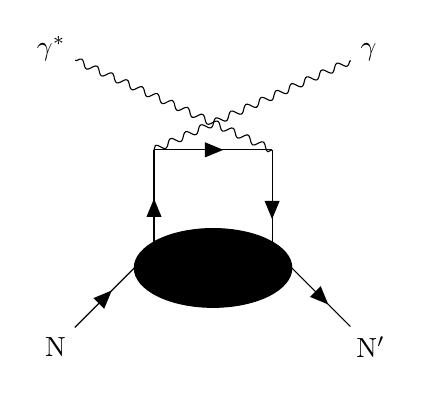
\begin{tikzpicture}
      \begin{feynman}
         \vertex (p1) at (0,0) {N};
         \vertex[above right=1cm and 2.0cm of p1] (a2) { };
         \vertex[below right=1cm and 2.0cm of a2] (p2) {N\(^{\prime}\)};

         \vertex[above left =0.00cm and 1.00cm of a2] (a20);
         \vertex[above left =0.00cm and 0.75cm of a2] (a21);
         \vertex[above left =0.25cm and 0.50cm of a2] (a22);
         \vertex[above left =0.25cm and 0.25cm of a2] (a23);
         \vertex[above right=0.25cm and 0.25cm of a2] (a24);
         \vertex[above right=0.25cm and 0.50cm of a2] (a25);
         \vertex[above right=0.00cm and 0.75cm of a2] (a26);
         \vertex[above right=0.00cm and 1.00cm of a2] (a27);

         \vertex[above =1.5cm of a21] (q0);
         \vertex[above =1.5cm of a26] (q1);

         \vertex[above left =1cm and 1cm of q0] (e0){\(\gamma^{*} \)};
         \vertex[above right=1cm and 1cm of q1] (e1){\(\gamma \)};

         \draw[fill,black] (a2) ellipse (1cm and 0.5cm);
         \diagram* {
            (p1) -- [fermion] (a20),
            (a27) -- [fermion] (p2),
            (a21) -- [fermion] (q0) -- [fermion](q1) -- [fermion](a26),
            (e0) -- [photon] (q1),
            (e1) -- [photon] (q0),
         };
      \end{feynman}
   \end{tikzpicture}
\end{center}

\begin{center}
   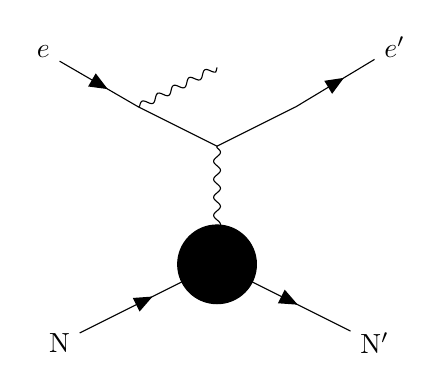
\begin{tikzpicture}
      \begin{feynman}
         \vertex (p1) at (0,0) {N};
         \vertex[above right=1cm and 2.0cm of p1] (a2) { };
         \vertex[below right=1cm and 2.0cm of a2] (p2) {N\(^{\prime}\)};

         \vertex[above left =0.00cm and 1.00cm of a2] (a20);
         \vertex[above left =0.00cm and 0.75cm of a2] (a21);
         \vertex[above left =0.25cm and 0.50cm of a2] (a22);
         \vertex[above left =0.25cm and 0.25cm of a2] (a23);
         \vertex[above right=0.25cm and 0.25cm of a2] (a24);
         \vertex[above right=0.25cm and 0.50cm of a2] (a25);
         \vertex[above right=0.00cm and 0.75cm of a2] (a26);
         \vertex[above right=0.00cm and 1.00cm of a2] (a27);

         \vertex[above =1.5cm of a2] (q0);

         \vertex[above left =0.5cm and 1cm of q0] (e01);
         \vertex[above left =1.0cm and 2cm of q0] (e0){\(e\)};
         \vertex[above right=1.0cm and 2cm of q0] (e1){\(e^{\prime}\)};
         \vertex[above right=0.5cm and 1cm of q0] (e11);

         \vertex[above right=0.5cm and 1.0cm of e01] (q1);

         \draw[fill,black] (a2) ellipse (0.5cm and 0.5cm);

         \diagram* {
            (p1) -- [fermion] (a2),
            (a2) -- [fermion] (p2),
            (e0) -- [fermion] (e01) -- [plain] (q0) -- [plain] (e11) -- 
            [fermion] (e1),
            (q0) -- [photon] (a2),
            (e01) -- [photon] (q1),
         };
      \end{feynman}
   \end{tikzpicture}
\end{center}

\begin{center}
   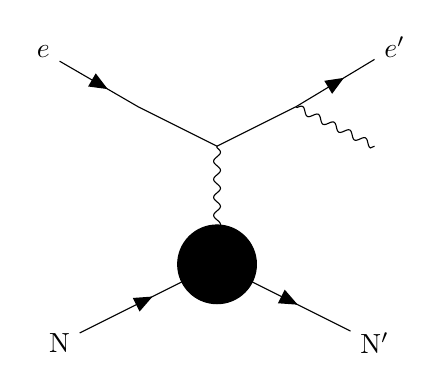
\begin{tikzpicture}
      \begin{feynman}
         \vertex (p1) at (0,0) {N};
         \vertex[above right=1cm and 2.0cm of p1] (a2) { };
         \vertex[below right=1cm and 2.0cm of a2] (p2) {N\(^{\prime}\)};

         \vertex[above left =0.00cm and 1.00cm of a2] (a20);
         \vertex[above left =0.00cm and 0.75cm of a2] (a21);
         \vertex[above left =0.25cm and 0.50cm of a2] (a22);
         \vertex[above left =0.25cm and 0.25cm of a2] (a23);
         \vertex[above right=0.25cm and 0.25cm of a2] (a24);
         \vertex[above right=0.25cm and 0.50cm of a2] (a25);
         \vertex[above right=0.00cm and 0.75cm of a2] (a26);
         \vertex[above right=0.00cm and 1.00cm of a2] (a27);

         \vertex[above =1.5cm of a2] (q0);

         \vertex[above left =0.5cm and 1cm of q0] (e01);
         \vertex[above left =1.0cm and 2cm of q0] (e0){\(e\)};
         \vertex[above right=1.0cm and 2cm of q0] (e1){\(e^{\prime}\)};
         \vertex[above right=0.5cm and 1cm of q0] (e11);

         \vertex[below right=0.5cm and 1.0cm of e11] (q1);

         \draw[fill,black] (a2) ellipse (0.5cm and 0.5cm);

         \diagram* {
            (p1) -- [fermion] (a2),
            (a2) -- [fermion] (p2),
            (e0) -- [fermion] (e01) -- [plain] (q0) -- [plain] (e11) -- 
            [fermion] (e1),
            (q0) -- [photon] (a2),
            (e11) -- [photon] (q1),
         };
      \end{feynman}
   \end{tikzpicture}
\end{center}

\begin{center}
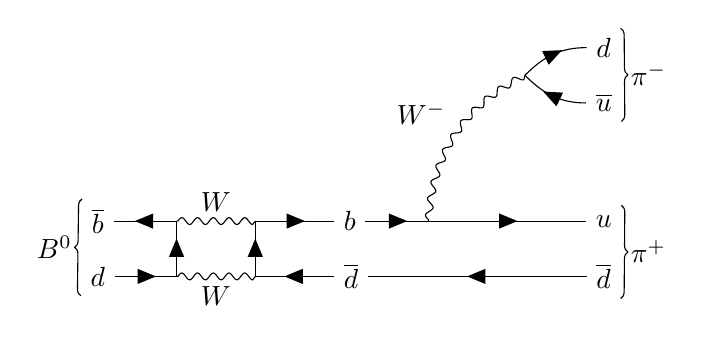
\begin{tikzpicture}
  \begin{feynman}
    \vertex (a1) {\(\overline b\)};
    \vertex[right=1cm of a1] (a2);
    \vertex[right=1cm of a2] (a3);
    \vertex[right=1cm of a3] (a4) {\(b\)};
    \vertex[right=1cm of a4] (a5);
    \vertex[right=2cm of a5] (a6) {\(u\)};

    \vertex[below=2em of a1] (b1) {\(d\)};
    \vertex[right=1cm of b1] (b2);
    \vertex[right=1cm of b2] (b3);
    \vertex[right=1cm of b3] (b4) {\(\overline d\)};
    \vertex[below=2em of a6] (b5) {\(\overline d\)};

    \vertex[above=of a6] (c1) {\(\overline u\)};
    \vertex[above=2em of c1] (c3) {\(d\)};
    \vertex at ($(c1)!0.5!(c3) - (1cm, 0)$) (c2);

    \diagram* {
      {[edges=fermion]
        (b1) -- (b2) -- (a2) -- (a1),
        (b5) -- (b4) -- (b3) -- (a3) -- (a4) -- (a5) -- (a6),
      },
      (a2) -- [boson, edge label=\(W\)] (a3),
      (b2) -- [boson, edge label'=\(W\)] (b3),

      (c1) -- [fermion, out=180, in=-45] (c2) -- [fermion, out=45, in=180] (c3),
      (a5) -- [boson, bend left, edge label=\(W^{-}\)] (c2),
    };

    \draw [decoration={brace}, decorate] (b1.south west) -- (a1.north west)
          node [pos=0.5, left] {\(B^{0}\)};
    \draw [decoration={brace}, decorate] (c3.north east) -- (c1.south east)
          node [pos=0.5, right] {\(\pi^{-}\)};
    \draw [decoration={brace}, decorate] (a6.north east) -- (b5.south east)
          node [pos=0.5, right] {\(\pi^{+}\)};
  \end{feynman}
\end{tikzpicture}
\end{center}

\end{document}
